\chapter{Requirement Analysis}
  \label{reqana}
  We will refer to AutoWDS in its current form as AutoWDS basic and the improved system, with the features of this requirements analysis realized, 
  is called AutoWDS extended.
  Up to now AutoWDS basic automatically uses just one or a random set of channels for its backbone wireless connections. 
  Additionally the topology it creates often reassembles a tree-like structure, since the APs connect themselves 
  to the first \ac{AP} which comes into range and additionally there are no fallbacks, if a link fails. 
  This results not only in severe bottlenecks for throughput, but also to prolonged downtimes, if a link happens to fail, since
  it takes some time for the APs to fully reconnect to the network Although the APs automatically rejoin the network if possible, 
  it results in an unnecessarily long downtime for the attached clients to this part of the network that has been disconnected. 
  Especially clients that depend on an uplink connection severely suffer from this lack of alternative/backup links. 
  The following requirements were therefore expressed to tackle these shortcomings.
  
  \begin{figure}[h!]
    \centering
    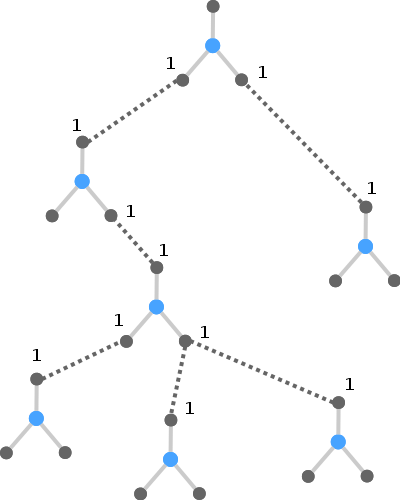
\includegraphics[width=0.3\columnwidth]{figures/autowds_basic_graph}
    \caption{AutoWDS basic network topology and channel assignment}
    \label{fig:autowds_basic_graph}
  \end{figure}

  \section{Increase Throughput}
  \label{reqincreasethroughput}
  Since the systems, which are connected to the APs, consume more data every day and with an increasing storage-footprint of new media like streaming \ac{HD} videos
  and generally downloading files of up to gigabytes, a wireless system is often solely defined by its capability of moving quantities of data over the air to the clients.
  This greed for throughput is amplified by an increasing number of devices that take part in radio communication, 
  thus it is also the key metric for quality in AutoWDS. 
  Furthermore not a single stream of data should be granted exclusive access to the radio, but
  many streams in parallel (gateway to clients) and also across the network (clients to clients), 
  as the common mesh / gateway / internet scenario does exist, but not exclusively (gateway to one client),
  since some usecases do only require local communication within the network.
  
  \section{Reduce End-to-end Link Failures}
  \label{regendtoend}
  AutoWDS basic is due to its tree-like structure very susceptible to network partition.
  As this may be just an inconvenience to users of devices like cellphones or laptops who are running non ciritical programs, 
  keeping up a connection to certain parts of the network in an industrial environment gains importance where for example heavy machines depend on its uplink connection in order 
  to continue proper operation. Hence AutoWDS extended has to provide the possibility to create and optionally use
  redundant connections in the network topology. The failing scenario is defined as one link breaks while others are still usable.
  A resulting network topology should have the possibility of having the 2-edge-connected attribute, as it may no be needed in all cases.
  
  \section{Utilize Variable Number of Radios}
  \label{utilvarnumradio}
  AutoWDS extended is currently planned to operate with only up to about 100 or less APs with a variable amount of radio-modules per \ac{AP}.
  Current versions of APs are equipped with one up to three radios each. It is supposed to work in heterogenous environments with 
  different numbers of radio-modules per \ac{AP}. As a consequence the available radio modules 
  should be utilized to achieve gains in overall throughput instead of finding an optimal solution which just uses one radio, as this solution is
  still inferior compared to a solution that utilizes multiple radios.
  Switching channels in short intervals to serve more than one channel is explicitly not desired as this leads to packet loss and latency for those channels the radio
  currently not services.
  
  \section{Use Variable Channel-sets for Assignment}
  AutoWDS extended will be used in variable environments and hence may face diverse restrictions with respect to the channels that are allowed to be used.
  Thus AutoWDS extended must accept a list of channels only of which it may choose from for channel assignment.
  
  \section{Restrictions}
    The new solution has also to be able to operate under the following restrictions:
    \begin{itemize}
     \item Centralized Computation and Configuration
     \item Static Environment
     \item Data Link Layer (layer 2) Usage
     \item Economic Constraints
    \end{itemize}
    
    \subsection{Centralized Computation and Configuration}
      AutoWDS extended must also be able to compute its solution on a central entity in contrast to a distributed fashion.
      Especially the APs should not be used to compute such a solution as no additional tasks are to be assigned to them.
      Although not currently planned, a potential algorithm may be included in the \ac{WLC} in the future.
      
      Reconfiguration of APs and collection of data from the \ac{AP}-network will only be able through a central \ac{WLC}.
      That means the potential network-topology and channel assignment solution has to be set on the \ac{WLC} and may not be broadcasted or otherwise
      distributed by or through the APs initially. The reason for such a focus on centralized taks is to provide the administrator the 
      opportunity to intervene and set manual wireless connections and other options, which is not as easily feasible in a distributed setup. 
      Additionally the management of certificates for security purposes is built up hierarchically and executed by the central \ac{WLC}.
      Especially since the support for doing things in a distributed fashion in the APs and WLCs (like ad-hoc-mode) is missing and would have to be implemented, 
      makes distributed approaches undesirable.
      
    \subsection{Static Environment}
      AutoWDS basic and extended is and will be designed for a static environment of APs. That means there will be no highly frequent changes in
      network topology or in link-quality. Although this does not completely render APs immobile, changes if any are expected to be very slow and gradually.
      
    \subsection{Data Link Layer (layer 2) Usage}
      The solution has to enable communication on layer 2, as some use cases do not use layer 3 (\ac{IP}) for their communication.
      Note that also a tunnel-mechanism (like ingress / egress in \ac{MPLS} \cite{mpls}), 
      where ethernet frames are encapsulated in a layer 3 packet for transportation and then later unpacket when delivering to the destination,
      is not preferred as this mechanism is currently not implemented in \ac{LCOS}.
    
    \subsection{Economic Constraints}
      Neither the central entity nor the APs are limited regarding power consumption. 
      Both will be permanently connected to the power grid and there is no power saving mode which could affect the design or computation.
      AutoWDS extended has to be able to find a solution on demand and in a short timeframe.
  